\subsection{Redes de Sensores Sem Fio}

\subsubsection{Contextualização}

A revista \emph{Business Week}, em setembro de 1999, elegeu a teconologia de micro-sensores em rede como uma das 21 tecnologias mais importantes do século XXI.
Uma rede de sensores é composta por dispositivos baratos e inteligentes com diversos sensores a bordo, conectados através de enlaces sem fio e em alguns casos conectados também à internet. Nós sensores podem ser distribuídos em grande quantidade e prover capacidades para se medir e controlar os mais diversos ambientes. \cite{Chong2003}

Cada nó sensor de uma rede é capaz de interagir com o ambiente em que se encontra inserido através do sensoriamento ou do controle de parâmetros físicos. Cada nó deve colaborar para cumprir as tarefas de rede pelo fato de usualmente um único nó apresentar capacidade computacional reduzida. Para se alcançar esta colaboração são utilizados enlaces de comunicação sem fio. Esta tecnologia oferece suporte para os mais variados tipos de aplicação e apresenta grandes desafios para as pesquisas em ciência da computação e engenharia. \cite{Holger2005}

Diversos modelos e tipos de sensores podem ser acoplados aos diferentes nós, conferindo habilidades aos nós para que realizem operações de monitoramento, rastreamento, vigilância e diversas outras tarefas relacionadas à detecção de enventos e mensurações do ambiente. A maior parte das baterias utilizadas para a operação destas redes não é recarregável, portanto, operações com baixo consumo de energia são uns dos maiores desafios neste contexto.\cite{Aboelaze2005}

As bases para o desenvolvmento das \rssfs advém de três principais áreas: sensoriamento, comunicação e computação (hardware, software a algoritmos). Logo, os avanços de cada uma destas áreas (em conjunto ou separadas) têm direcionado a pesquisa em \rssf. \cite{Chong2003}


\paragraph{Tipos de Aplicações}
O desenvolvimento das \rssfs oferece suporte para uma grande variedade de aplicações, principalmente em casos de detecção de parâmetros em ambientes. Aplicações militares, detecção de incêndios, monitoramento de fábricas, recuperação de desastres, agricultura de precisão, etc; são exemplos de aplicações de \rssfs.

\cite{Holger2005} definem quatro principais padrões de operação em redes de sensores. Estes padrões de operações definem os principais tipos de aplicação.

\begin{description}

\item[Detecção de Eventos:] São casos onde os nós sensores devem reportar a detecção de ocorrência de um dado evento de interesse. O caso mais simples de detecção de evento é quando um único nó detecta um evento (algum limite pré-definido é ultrapassado) e deve reportar aos outros nós. Casos mais complexos são os que requerem consenso de vários nós para se determinar a ocorrência de um determinado evento.

\item[Medidas Periódicas: ] São as situações em que os nós têm tarefas somente de medições, reportando periodicamente as informações coletadas. Em alguns casos, estes relatórios podem ser enviados em casos de detecção de eventos. Porém, os critérios sobre os momentos de relatório devem ficar a critério das aplicações.

\item[Aproximação de Funções e Detecção de Bordas:] Um \rssf pode utilizar amostras de diferentes regiões para estimar parâmetros gerais do ambiente. Um exemplo é o modo como os valores físicos de leitura de temperatura pode variar de uma região para outra. Neste caso, ignorando outros fatores condicionantes, pode-se supor que a medida da temperatura pode ser dada em função da localização. Em consequencia disto, podem ser utilizadas amostragens de temperatura de diferentes regiões para se aproximar esta função desconhecida.

\item[Rastreamento:] A causa de um evento pode ser móvel, como casos de entrada de intrusos em cenários de vigilância. A \rssf pode ser configurada para relatar as atualizações da posição corrente do intruso. Existe também a possibilidade de se estimar a velocidade e direção dos intrusos. 

\end{description}



\subsubsection{Características}
Redes de sensores podem apresentar diferentes características e requisitos. Cada rede apresentará características variadas, pois cada aplicação pode demandar diferentes requisitos.
Este fato obriga a rede de sensores a se preocuparem com fatores específicos.

\cite{Loureiro} discute algumas características mais relevantes:

\begin{description}
	\item[Endereçamento dos nós sensores:] Trata-se de endereçar unicamente um sensor dentro da rede. Existem casos em que se torna necessário saber a localização ou fonte dos dados, como quando são utilizados sensores espalhados em uma fábrica ou no corpo humano. Nesses casos é interessante saber a fonte dos dados. Contudo, em casos onde existe uma infinidade de sensores medindo valores no ambiente pode não ser necessário identificar cada nó individualmente.

	\item[Agregação dos dados:] Indica a possibilidade da rede agregar os dados coletados pelo sensor. Ou seja, se os dados serão condesados em um único ponto, ou se serão espalhados e enviados por todos os nós. Se esta funcionalidade (agregação) estiver presente, cria-se a possibilidade de economia de tráfego de mensagens até uma estação base.

	\item[Mobilidade dos Sensores: ] Preocupa-se com a mobilidade ou não dos sensores em relação aos sistemas em que se encontram inseridos. Diferentes abordagens devem ser utilizadas em cada caso. 

	\item[Quantidade de Sensores:] Aplicações de \rssf podem conter de poucos, à dezenas e à milhares de nós sensores. Uma das maiores preocupações, neste caso, é a escalabilidade do sistema. Combinada com a mobilidade, esta questão pode ser uma das características mais críticas no desenvolvimento de uma aplicação de \rssf.

	CONTINUAR AQUI.. AINDA NAO ACABOU!

\end{description}


mostrar as classificações das tabelas do capitulo do Luiz

pagina 9 do holger

\subsubsection{Nós Sensores}

O hardware de um nó sensor da rede é composto por um microprocessador, uma unidade de armazenamento, sensores, conversores analógico-digital, um transceiver de dados, controladores que unem estas partes, e uma fonte de energia. \cite{Culler2004}

Segundo \cite{Holger2005}, os requisitos das aplicações representam fatores decisivos no que diz respeito a tamanho, custos, e consumo de energia dos nós. Características tais como comunicação e poder de processamento devem ser prover um nível mínimo de qualidade que atenda aos requisitos destas aplicações. Encontrar o equilíbrio entre funcionalidades e custos é uma tarefa crucial na escolha do modelo de nó correto.

\cite{Holger2005} definem a estrutura básica de um nó sensor sem fio como:
\begin{description}
\item[Controlador:] Um controlador para processar os dados, capaz de executar códigos arbitrários.
\item[Memória:] Unidade de memória para armazenar programas e alguns dados intermediários.
\item[Sensores e Autuadores:] A verdadeira interface com o mundo real, dispositivos que podem observar ou controlar parâmetros físicos do ambiente.
\item[Fonte de Energia:] Componente responsável por suprir as necessidades de energia do nó sensor.
\end{description}

Cada um destes componentes deve trabalhar em busca de alcançar o equilíbrio entre o menor gasto de energia possível e a necessidade de cumprir sua tarefa com um mínimo de qualidade.

\begin{figure}
\centering
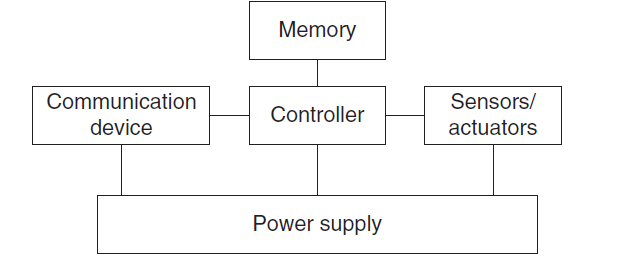
\includegraphics[width=10cm]{pictures/overview_node.png}
\caption{Visão Geral do Hardware de um Nó Sensor Sem Fio}
 \label{fig:overview}
\end{figure}

\paragraph{algum modelo de nó}

Lorem ipsum dolor sit amet, consectetur adipiscing elit. Donec mauris turpis, facilisis sed malesuada a, sollicitudin vel ligula. Aliquam porttitor augue nec massa sollicitudin adipiscing. Curabitur consequat sagittis metus ut sollicitudin. Duis mi ipsum, fermentum quis scelerisque quis, ultricies non eros. Vestibulum fringilla felis vel tortor malesuada consectetur. Nullam velit mi, porta id imperdiet ac, ornare sit amet orci. Praesent fringilla, turpis quis fringilla molestie, risus metus iaculis nisi, placerat tempus velit ante quis justo. Fusce sit amet ante dui. Aenean et nisl eu metus cursus luctus non ut lorem. Ut dignissim euismod aliquam. Nunc quis risus odio, nec auctor nunc. Nam non malesuada turpis.

Vestibulum sit amet tortor nunc. Nunc rhoncus accumsan dictum. Duis ac felis nunc, molestie porta metus. Pellentesque sollicitudin nulla eget nibh dictum quis cursus nisi condimentum. Curabitur at dui sit amet orci dapibus cursus. Suspendisse vitae arcu sed metus dignissim molestie. Fusce euismod laoreet lectus, id elementum nisi luctus ac. Morbi massa odio, auctor eget commodo tristique, condimentum non diam. Sed feugiat laoreet porta. Suspendisse commodo dapibus lobortis. Sed feugiat adipiscing est, quis malesuada mi imperdiet vitae. Ut et blandit nibh.

\paragraph{algum outro modelo}
Vivamus at tortor lacus, vel blandit orci. Proin vitae posuere metus. Morbi ante ligula, sollicitudin ut ullamcorper quis, elementum ullamcorper diam. Cras id tortor quam, eget fringilla urna. Nullam vitae nibh quam, at congue arcu. Nullam dolor tortor, tristique sed viverra vitae, vulputate ac nunc. Duis convallis nisi sed justo tristique nec vestibulum metus mattis. Suspendisse potenti. Quisque porta condimentum odio, ac pulvinar libero molestie vel. Aenean blandit rutrum nisl eget feugiat. Nunc sollicitudin leo vitae neque rhoncus commodo. Fusce gravida sapien ut ligula posuere et mattis nulla euismod. Vestibulum ante ipsum primis in faucibus orci luctus et ultrices posuere cubilia Curae; Vivamus venenatis leo nunc. Nunc id orci metus. Cum sociis natoque penatibus et magnis dis parturient montes, nascetur ridiculus mus. Cras posuere sapien sit amet nisl rhoncus eget sodales diam tristique. Quisque bibendum imperdiet dictum. Nulla eget neque magna.

Phasellus posuere, orci quis sagittis malesuada, turpis urna fermentum metus, ac porttitor massa dolor cursus dui. In eget nisi at mauris tincidunt accumsan non ac justo. Mauris libero nunc, commodo nec consequat ut, vestibulum eu enim. Nullam interdum adipiscing dui, eu elementum massa sodales at. Nam ipsum neque, dignissim non euismod non, fermentum at mauris. Morbi eros ante, malesuada eget euismod et, commodo ac elit. Donec mauris ligula, tempor at dapibus eu, dapibus in est. Donec egestas velit sed mauris tristique molestie ultrices turpis semper. Phasellus elit enim, porttitor sed volutpat eget, varius vitae sem. Aliquam consequat quam eu diam venenatis non congue lacus pharetra. Class aptent taciti sociosqu ad litora torquent per conubia nostra, per inceptos himenaeos. Donec sapien sapien, suscipit nec euismod eget, lobortis vitae tortor. Vivamus eget vulputate nulla. Fusce sem turpis, condimentum vel elementum a, pretium vitae quam. Maecenas sit amet mauris nibh. Phasellus sit amet augue leo. 


\paragraph{um terceiro modelo}
Vivamus at tortor lacus, vel blandit orci. Proin vitae posuere metus. Morbi ante ligula, sollicitudin ut ullamcorper quis, elementum ullamcorper diam. Cras id tortor quam, eget fringilla urna. Nullam vitae nibh quam, at congue arcu. Nullam dolor tortor, tristique sed viverra vitae, vulputate ac nunc. Duis convallis nisi sed justo tristique nec vestibulum metus mattis. Suspendisse potenti. Quisque porta condimentum odio, ac pulvinar libero molestie vel. Aenean blandit rutrum nisl eget feugiat. Nunc sollicitudin leo vitae neque rhoncus commodo. Fusce gravida sapien ut ligula posuere et mattis nulla euismod. Vestibulum ante ipsum primis in faucibus orci luctus et ultrices posuere cubilia Curae; Vivamus venenatis leo nunc. Nunc id orci metus. Cum sociis natoque penatibus et magnis dis parturient montes, nascetur ridiculus mus. Cras posuere sapien sit amet nisl rhoncus eget sodales diam tristique. Quisque bibendum imperdiet dictum. Nulla eget neque magna.

Phasellus posuere, orci quis sagittis malesuada, turpis urna fermentum metus, ac porttitor massa dolor cursus dui. In eget nisi at mauris tincidunt accumsan non ac justo. Mauris libero nunc, commodo nec consequat ut, vestibulum eu enim. Nullam interdum adipiscing dui, eu elementum massa sodales at. Nam ipsum neque, dignissim non euismod non, fermentum at mauris. Morbi eros ante, malesuada eget euismod et, commodo ac elit. Donec mauris ligula, tempor at dapibus eu, dapibus in est. Donec egestas velit sed mauris tristique molestie ultrices turpis semper. Phasellus elit enim, porttitor sed volutpat eget, varius vitae sem. Aliquam consequat quam eu diam venenatis non congue lacus pharetra. Class aptent taciti sociosqu ad litora torquent per conubia nostra, per inceptos himenaeos. Donec sapien sapien, suscipit nec euismod eget, lobortis vitae tortor. Vivamus eget vulputate nulla. Fusce sem turpis, condimentum vel elementum a, pretium vitae quam. Maecenas sit amet mauris nibh. Phasellus sit amet augue leo. 
